\documentclass{article}

% For Unicode support
\usepackage{xeCJK}

% Title sec
\usepackage{titlesec}

% APA Citation
\usepackage[
  style           = apa,
  citestyle       = authoryear,
  sorting         = nyt,
  sortcites       = true,
  autocite        = inline,
  citetracker     = false,
  maxbibnames     = 99,
  maxcitenames    = 2,
  backend         = biber,
  isbn            = false,
  doi             = true,
  urldate         = short,
  backend         = biber,
  defernumbers    = true
]{biblatex}

\DeclareBibliographyCategory{printcite}
\newcommand{\printcite}[1]{%
  \addtocategory{printcite}{#1}%
  \defbibcheck{key#1}{
    \iffieldequalstr{entrykey}{#1}
    {}
  {\skipentry}}%
  \printbibliography[heading=none,check=key#1]%
}
\addbibresource{cite.bib}

% Provide support on formatting SI Unit
\usepackage{siunitx}
\sisetup{per-mode=fraction}

% Math package
\usepackage{amsmath}
\renewcommand{\frac}{\dfrac}

\newcounter{source}
\newcommand{\sourcemeta}[3]{\subsection{Student Researcher} #1 %
  \subsection{Type} #2 %
\subsection{Citation} \printcite{#3}}

\newcommand{\source}[3]{\stepcounter{source} %
  \section{Source \#\thesource} %
\sourcemeta{#1}{#2}{#3}}

% Customized reflection entry
\newcounter{reflection}
\newcommand{\reflection}[2]{\stepcounter{reflection} %
\section*{Reflection \#\thereflection}
  %\noindent Log what you have done, what you have discovered, what you have learned, what are your next steps\ldots 

\paragraph{Date} #1

  \vspace*{-0.5cm}
\paragraph{Initials} #2}

% Customized reference
\usepackage[hidelinks]{hyperref}

% Better typesetting
\usepackage{microtype}

% Menukeys
\usepackage[os=win]{menukeys}

% Table
\usepackage{tabularx}
\usepackage{booktabs}
\usepackage{multirow}
\usepackage{makecell}
\newcolumntype{b}{>{\centering\arraybackslash}X}
\newcolumntype{s}{>{\hsize=.4\hsize\centering}X}

% Float
\usepackage{newfloat}

% 1.5 line spacing
\usepackage{setspace}
\setstretch{2.0}

% Subfigure
\usepackage{subcaption}
\usepackage{caption}

% Finer geometry
\usepackage{geometry}
\geometry{a4paper}

% Define some constants
\renewcommand{\title}{Project WORLEY}

% Define field input, i.e., box
\usepackage[most]{tcolorbox}
\newenvironment{field}{\begin{tcolorbox}[%
    enhanced, 
    breakable, 
    colback = white, colframe = black,
    sharp corners,
    boxrule = 0pt, bottomrule = 1pt, toprule = 1pt,
    leftrule = 0.5pt, rightrule = 0.5pt
]{}}{\end{tcolorbox}}

% Hanging indent
\usepackage{hanging}

% Enhanced list
\usepackage{enumitem}
\setitemize{noitemsep}
\setenumerate{noitemsep}

% Reset section number within part
\usepackage{chngcntr}
\counterwithin*{section}{part}

% Footer
\usepackage{fancyhdr}
\pagestyle{fancy}
\fancyhf[FR]{\hyperlink{toc}{Return to Table of Contents}}

% Glossary acronym
\usepackage[acronym]{glossaries}
\makenoidxglossaries
% dof
\newacronym{dof}{DoF}{degrees of freedom}
% ghp
\newacronym{ghp}{GHP}{Governor's Honors Program}
% rpi
\newacronym{rpi}{RPI}{Raspberry Pi}
% gpio
\newacronym{gpio}{GPIO}{General Purpose Input/Output}
% udp
\newacronym{udp}{UDP}{User Datagram Protocol}
% asr
\newacronym{asr}{ASR}{Automatic Speech Recognition}
% ml
\newacronym{ml}{ML}{Machine Learning}
% asl
\newacronym{asl}{ASL}{American Sign Language}
% gosa
\newacronym{gosa}{GOSA}{Georgia Office of Student Achievement}
% cad
\newacronym{cad}{CAD}{computer-aided design}
% sd
\newacronym{sd}{SD}{speaker diarization}
% vad
\newacronym{vad}{VAD}{voice activation detection}
% stt
\newacronym{stt}{STT}{speech-to-text}
% mvp
\newacronym{mvp}{MVP}{minimum viable product}
% cs
\newacronym{cs}{CS}{computer science}
% Table of contents title change
\renewcommand{\contentsname}{Table of Contents}

% Part and Subpart only
\setcounter{tocdepth}{-1}

\begin{document}
\begin{titlepage}
  \centering
  \vspace*{1in}
  \begin{tikzpicture}[overlay,remember picture]
    \node[anchor=center, opacity=0.15] at (current page.center) {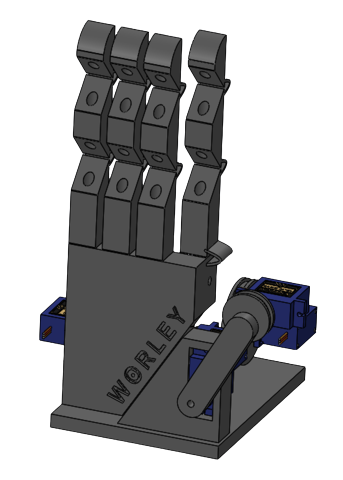
\includegraphics[width=0.8\paperwidth]{img/cad/hand.png}};
  \end{tikzpicture}
  {\fontsize{56pt}{2\baselineskip}\selectfont \bfseries
  \title}
  \vfill

  \Large
  GOSA Governor's Honors Program 60\\
  Statesboro, Georgia

  \vspace{0.5in}
  \setstretch{1.15}\selectfont

  \vspace{1em}
  \textbf{Team Leader}\\ Anish Goyal

  \vspace{1em}
  \textbf{Team Members}\\ Yubo Cao \& Ian Oberbeck

  \vspace{1em}
  \textbf{Teachers}\\ Kai Ouyang, Craig Worley,  Anupam Goli, \& Dejah Crossfield
\end{titlepage}
\tableofcontents
\newpage

\part{Directions and Tips}

Delete this entire page before submitting FINAL logbook check (not before)

\begin{itemize}
\item Remember that this is a legal document.
\item Anyone should be able to follow exactly what you did in your project by
    reading your logbook. That's the level of detail you need.
\item You MAY NOT delete any entries/data from this notebook. If you need to
    delete anything, you should strike through it (\menu{format > text >
    strikethrough})
    . You can also make multiple versions of your entries, if appropriate.
\item If you did work on other documents, you may cut and paste the items from
    those other locations. Just provide citations/reference those other
    locations. If you can't cut \& paste easily (like you are referencing a
    physical lab notebook), you should decide if it's important to scan in the
    document or to just reference your previous work.
\end{itemize}

EVERY SKETCH OR DESIGN OR CODE you create should be included in your journal.
Every design change must be documented. If you have any physical lab set ups or
things you are building, include photos in your reflection entries. You must
have AT LEAST SOME PICTURES that include you doing work on your project.

\begin{itemize}
    \item Every day you work on a project, you should include a reflection entry
        with a summary of what you accomplished that day, any ideas you
        discussed, and other important ideas (even if you're not sure and are
        just considering them).
    \item Use your reflection entries to plan out what your next day should
        accomplish.
    \item At some point, you will need to do project planning, and you should
        include images of your project planning document (like a kanban board in
        your journal).
    \item Research/bibliography pages should be set up correctly using proper.
    \item If appropriate, title your entries (not reflection entries but other
        items in your lab notebook). You can insert ADDITIONAL sections in your
        logbook, but you must have everything in the template.
    \item Date all entries and put your initials. If you modify the entry, put
        modified dates and re-initial. You can also make version 1, 2, etc. for
        entries.
Include page numbers
\end{itemize}

\part{Brainstorming}

\begin{itemize}
    \item A robotic hand that can act out American Sign Language (ASL) can be used for someone who relies on ASL as their primary communication language to be able to communicate independently, without relying on another person to interpret.
    \item The idea is further extended to a robotic arm that can act out ASL, which can be used to teach ASL to people who are interested in learning it.
    \item Finally, more research made us realize ASL is a language on its own, and it is not a direct translation of English. Therefore, we decided to make a robotic arm that can act out ASL, and also translate English to ASL using a BERT model.
\end{itemize}
\addtocontents{toc}{\protect\hypertarget{toc}{}}
\part{Research}

\part{Reflection}
\reflection{7/1/2023}{Anish Goyal}

For our \href{https://gosa.georgia.gov/governors-honors-program}{\gls{gosa} \gls{ghp}} final engineering project, we wanted to create an innovative device that could improve the lives of others. Our best friend, Cory, suffers from hearing loss and has to use hearing aids or sign language to communicate properly. This inspired us to create an application that signs out the \gls{asl} alphabet using a mechanical robot hand from voice input in real time.

Even though it's the first day, we have already faced skepticism from our engineering instructors regarding our ability to achieve ten \gls{dof} within a tight timeframe of two weeks. However, this skepticism has only fueled our determination to prove them wrong.

Here is some of the stuff we came up with during our brainstorming session today:
\begin{description}
\item[Pybluez] This Python library allows us to establish a Bluetooth connection between the computer controller and the \gls{rpi}-controlled robot hand. It also provides an interface to seamlessly communicate with the hand.

\item[RPI GPIO programming] To interface with the robot hand, we leveraged \gls{rpi}'s \gls{gpio} pins. By connecting our servos to pins, we will be able to control the hand's actuators and enable precise finger movements.

\item[UDP and Custom audio transmission protocol] We want to implement \gls{udp} to transmit audio data from the mobile application to the signal processing module. We could also design a custom audio transmission protocol to ensure efficient and reliable data transfer.

\item[Zero-copy memory-efficient thread-safe asynchronous queue] This concept will help us optimize the data processing pipeline by minimizing memory overhead and ensuring thread safety. By utilizing an asynchronous queue, we can achieve efficient parallel processing of audio data.

\item[Real time speech recognition through Whisper] We want to integrate cutting-edge techniques such as sliding window-based speech recognition and speaker diarization using the Whisper \gls{asr} model by OpenAI. Cutting the live audio into segments and feeding them into Whisper yields an accurate transcription of voice input with the illusion of real-time recognition.

\item[Kubeflow-powered ML operations] We want to employ Kubeflow, a \gls{ml} toolkit for Kubernetes, to build a robust \gls{ml} pipeline. With Kubeflow, we can ensure data provenance, making it possible to trace and understand the entire ML workflow.

[Ray cluster-powered hyperparameter tuning] Using Ray, an open-source framework for distributed computing to optimize our ML models, will greatly accelerate the process of hyperparameter tuning, enabling better feature recognition and extraction.
\end{description}

\reflection{7/3/2023}{Yubo Cao}

Over the past two days, we have been working on a presentation for the project pitch, \gls{cad} of the model, \& the preliminary testing of the servo motion. We also researched existing solutions on speech recognition, \gls{sd}, \gls{vad}, \& \gls{stt}. After our meeting with Mr. Kai, the \gls{cs} department head at \gls{ghp}, we have decided to focus on the implementation of the robotic finger and hand, creating a backlog \& \gls{mvp} list, and following an incremental goal structure to assure the project's success in the end.

\reflection{7/5/2023}{Yubo Cao}

For today, Ian worked on the 

\reflection{7/7/2023}{Yubo Cao}



\reflection{7/10/2023}{Anish Goyal}



\newpage
\part{Initial Proposal Form}

\section{Project Title}

Don't worry...you don't have to commit to this title!\\
\emph{No longer than 65 characters}

\begin{field}
  \title
\end{field}

Science/engineering fair project category

\begin{field}
  Robotics and Intelligent Machines (ROBO)
\end{field}

\section{Background Research}

\subsection{Rationale For Your Project}

What similar devices/technology/research studies have investigated similar ideas?

\begin{field}

\end{field}

\subsection{Why is this research project important/needed (background research needs to support this claim)?}

\emph{Explain any societal impact of your research/include any personal
connections to the project.}

\begin{field}

\end{field}

\subsection{Major science/engineering principles and concepts}


\emph{What you will need to understand to fully understand the scope of
your project.}

\begin{field}
  
\end{field}

\subsection{Objective (science project only) - start with big picture for now}

\emph{Provide context for your investigation with a need, who would be
  interested in your investigation, what you will test and vary, and what outcomes (relationships or trends) you expect to find.}

\begin{field}

\end{field}

\section{Methodology}

\emph{Science project: general procedure/timeline of events to test hypothesis}

\subsection{Independent variable and treatment levels}

\begin{field}
 
\end{field}

\subsection{Dependent variable to measure effects of change}

\begin{field}

\end{field}


\subsection{Control group to obtain baseline/source of comparison}

\begin{field}

\end{field}


\subsection{Sample size: trials per treatment level/total}

\begin{field}
  
\end{field}

\subsection{Materials/Equipment}

\emph{List key items that need to be ordered/purchased, the vendor, and
cost}

\begin{field}
 
\end{field}

\subsection{Procedures}

\emph{Big picture for now as you will need to conduct additional
research to streamline your procedure.}

\begin{field}
  
\end{field}


\section{References: APA}

\begin{field}

\end{field}



\addtocontents{toc}{\protect\setcounter{tocdepth}{2}}
\part{Initial Research Plan form 1A}

% TODO: See if need to be removed
\textbf{All projects must have a Research Plan}
\begin{enumerate}[label=\Alph*.]
    \item The Research Plan is to be written prior to experimentation following the instructions below to detail the rationale, research question(s), methodology, and risk assessment of the proposed research.
    \item If changes are made during the research, such changes can be added to the original research plan as an addendum, recognizing that some changes may require returning to the IRB or SRC for appropriate review and approvals. If no additional approvals are required, this addendum serves as a project summary to explain research that was conducted.
    \item If no changes are made from the original research plan, no project summary is required.
\end{enumerate}

% TODO: To be removed
% \textbf{The Research Plan/Project Summary should include the following}

\section{Rationale}

Include a brief synopsis of the background that supports your research problem and explain why this research is important and if applicable, explain any societal impact of your research.

\begin{field}
  
\end{field}

\section{Research Question}

\begin{field}
\end{field}

\section{Overall Hypothesis}

Include your independent and dependent variables AND justification for your hypothesis. Include a separate null hypothesis.

\subsection*{Hypothesis}

\begin{field}
\end{field}

\subsection*{Null Hypothesis}

\begin{field}
\end{field}

\section{Procedure}

Detailed procedures for your experimentation, including methods for data
collection, and when applicable, the source of data used.

\subsection{Independent Variable}
Including units and treatment levels to be tested

\begin{field}

\end{field}

\subsection{Dependent variable}
Including method of measurement and units

\begin{field}
   
\end{field}


\subsection{Control Group/Baseline defined with units}

\begin{field}

\end{field}

\subsection{Experimental controls}
Complete list of all variables that will remain constant between treatment levels

\begin{field}

\end{field}

\subsection{Materials/Tools/Equipment needed for testing (include quantities)}

\begin{field}
   
\end{field}

\subsection{Experimental procedure} 

Detail all procedures and experimental design including methods for data collection, and when applicable, the source of data used. This should be a numbered list, like you would have for a lab, specific enough for someone unfamiliar with your experiment to follow. Be sure to include the number of trials.

\begin{field}
  
\end{field}


\subsection{Risk and Safety}

Identify any potential risks and safety precautions needed.

\begin{field}

\end{field}

\subsection{Data Analysis}

Describe the procedures you will use to analyze the data/results. 

\begin{field}
   
\end{field}

\subsection{Bibliography}

List major references (e.g. science journal articles, books, internet sites) from your literature review.

\begin{field}
    \printbibliography[heading=none]
\end{field}

\part{Experimentation 1}

\section*{Dates of Experimentation}
List the dates over which the experimentation took place.

\begin{field}

\end{field}

\section{Notes}

Detailed observations about the process for your experiment. What is working
well? What needs to be improved on in your next experiment?

\begin{field}

\end{field}

\section{Data}

Include your raw data from your experiment, with dates.

\section*{Photos}

Include all photos of your experiment, with dates.

\section{Addendum}

Identify in detail any modifications you need to make to your experimental plan,
based on this round of experimentation.

\begin{field}

\end{field}
\part{Experimentation 2}

Depending on how your first round of experimentation worked, this could be
additional data collection using the same procedure, or it could be a fresh set
of experiments after modifying your procedure.

\section*{Dates of Experimentation}

List the dates over which the experimentation took place.

\begin{field}

\end{field}

\section{Notes}

Detailed observations about the process for your experiment. What is working
well? What needs to be improved on in your next experiment?

\begin{field}

\end{field}

\section{Data}

Include your raw data from your experiment, with dates.

\section*{Photos}

Include all photos of your experiment, with dates.

\section{Addendum}

Identify in detail any modifications you need to make to your experimental plan,
based on this round of experimentation.

\begin{field}

\end{field}

\addtocontents{toc}{\protect\setcounter{tocdepth}{1}}
\part{Data Tables \& Graphs}


\begin{description}
    \item[Data Table] Include both qualitative and quantitative summarized (not
        raw) data
    \item[Graph(s)] Graph should be structured in such a way that the effect of
        the independent variable upon the dependent variable can be easily
        understood. Display comparison between experimental groups and control
        group as well as to display trends (if applicable)
\end{description}

\part{Statistical Analysis}

\begin{description}
    \item[Hypothesis]
    \item[Type of statistical analysis (t-test, chi square test, ANOVA, etc)]
    \item[Degrees of freedom]
    \item[Critical Value]
    \item[P Value]
    \item[Summary statement] (The null hypothesis of \_\_\_ {was rejected/failed to be rejected} because \ldots [insert stats].
\end{description}


\part{Result \& Conclusion}

\begin{description}
\item[Claim] Answer original research question or state whether hypotheses are confirmed or rejected.


\item[Evidence] Summarize trends. Use numerical data with units, including averages, rates, statistical analysis, etc., in addition to using qualitative data (observations).


\item[Reasoning] How does your evidence support your claim (or not support it)? Include relevant research/scientific principles. If unsupported, why not? What errors may have occurred? What would you do differently?


\item[Application] Discuss practical applications of your research or findings. Include where you go from here...ideas for further study/research.
\end{description}

 
\nocite{*}

% print glossary
\printnoidxglossary[type=\acronymtype,title=Acronyms]
\newpage

% print bibliography
\printbibliography

\end{document} 